\section{Algorithm Design}
In this section, we wil talk about the design of the algorithms.
\subsection{Feature Design}
The problem can be simplified to a binary classification problem.
The input is the features of the data sets, and the output is the winner side (the radient or the dire).
The first group of features we can get from the match is the hero lineup.
In Dota, each team chooses 5 heroes and two teams cannot have the duplicate heroes.
Since the total number of heroes in Dota is 111, we can use 111 features to show the heroes using situation in a game.
For the value of features, 0 means no team picks up this hero;
1 means radiant team chooses this hero.
-1 means dire team chooses the hero.
The first 111 features and the corresponding heroes' names can be seen in Table~\ref{table:hero}

\begin{table}[!tb] 
\scriptsize
\centering \caption{Hero Table}
\label{table:hero} 
\begin{tabular} {|c|c|c|c|c|c|} 
\hline Name & ID & Name & ID & Name & ID
\\ \hline abaddon&0&io&37&rubick&74
\\ \hline alchemist&1&jakiro&38&sand-king&75
\\ \hline ancient-apparition&2&juggernaut&39&shadow-demon&76
\\ \hline anti-mage&3&keeper&40&shadow-fiend&77
\\ \hline arc-warden&4&kunkka&41&shadow-shaman&78
\\ \hline axe&5&legion-commander&42&silencer&79
\\ \hline bane&6&leshrac&43&skywrath-mage&80
\\ \hline batrider&7&lich&44&slardar&81
\\ \hline beastmaster&8&lifestealer&45&slark&82
\\ \hline bloodseeker&9&lina&46&sniper&83
\\ \hline bounty-hunter&10&lion&47&spectre&84
\\ \hline brewmaster&11&lone-druid&48&spirit-breaker&85
\\ \hline bristleback&12&luna&49&storm-spirit&86
\\ \hline broodmother&13&lycan&50&sven&87
\\ \hline centaur-warrunner&14&magnus&51&techies&88
\\ \hline chaos-knight&15&medusa&52&templar-assassin&89
\\ \hline chen&16&meepo&53&terrorblade&90
\\ \hline clinkz&17&mirana&54&tidehunter&91
\\ \hline clockwerk&18&morphling&55&timbersaw&92
\\ \hline crystal-maiden&19&naga-siren&56&tinker&93
\\ \hline dark-seer&20&natures-prophet&57&tiny&94
\\ \hline dazzle&21&necrophos&58&treant-protector&95
\\ \hline death-prophet&22&night-stalker&59&troll-warlord&96
\\ \hline disruptor&23&nyx-assassin&60&tusk&97
\\ \hline doom&24&ogre-magi&61&undying&98
\\ \hline dragon-knight&25&omniknight&62&ursa&99
\\ \hline drow-ranger&26&oracle&63&vengeful-spirit&100
\\ \hline earth-spirit&27&outworld-devourer&64&venomancer&101
\\ \hline earthshaker&28&phantom-assassin&65&viper&102
\\ \hline elder-titan&29&phantom-lancer&66&visage&103
\\ \hline ember-spirit&30&phoenix&67&warlock&104
\\ \hline enchantress&31&puck&68&weaver&105
\\ \hline enigma&32&pudge&69&windranger&106
\\ \hline faceless-void&33&pugna&70&winter-wyvern&107
\\ \hline gyrocopter&34&queen&71&witch-doctor&108
\\ \hline huskar&35&razor&72&wraith-king&109
\\ \hline invoker&36&riki&73&zeus&110
\\ \hline \end{tabular} 
\end{table}

\begin{table}[!tb] 
\footnotesize
\centering \caption{Synergic Relationship and Counter Relationship}
\label{table:pairs} 
\begin{tabular} {|c|c|c|c|} 
\hline \multicolumn{2}{|c|}{Synergic} & \multicolumn{2}{|c|}{Counter}
\\ \hline Hero ID & Hero ID & Hero ID & Hero ID
\\ \hline 33&2&2&1
\\ \hline 33&36&107&26
\\ \hline 49&76&79&32
\\ \hline 12&37&74&32
\\ \hline 108&33&76&42
\\ \hline 26&25&86&93
\\ \hline 104&20&3&52
\\ \hline 21&56&79&86
\\ \hline 30&54&60&52
\\ \hline 32&34&60&43
\\ \hline 21&35&60&86
\\ \hline 45&68&87&39
\\ \hline 81&89&87&89
\\ \hline 99&37&20&89
\\ \hline 42&36&18&83
\\ \hline 30&51&99&1
\\ \hline 40&66&76&3
\\ \hline 97&14&86&30
\\ \hline 8&36&72&64
\\ \hline 9&110&33&45
\\ \hline 62&64&29&55
\\ \hline 63&35&23&37
\\ \hline 62&65&74&91
\\ \hline 34&33&100&33
\\ \hline 94&37&84&26
\\ \hline 8&93&28&53
\\ \hline 67&33&89&36
\\ \hline 16&57&92&25
\\ \hline 6&54&31&16
\\ \hline 76&54&56&33
\\ \hline
\end{tabular}
\end{table}

In addition, we also consider the synergic relationship of heroes and counter relationship of heroes.
Synergic relationship means in one team, there are two heroes who cooperate with each other and
can get large advantage in the match.
Counter relationship indicates a hero in a team has a large advantage to another hero in the other team,
which means a hero can easily kill or uncomfort the enemy hero.
These two relationships play very significant role in the match.
When the relationship exists in the hero lineup, the balance of game result changed.
These two relationships are never considered in the previous research.
The number of these relationships are so many that we have to pickup some representative relationships.
In this research, we pickup 30 most influence synergic and counter hero pairs,
which can be seen in Table~\ref{table:pairs}
So, we have 30 features for synergic relationship and 30 features for counter relationship.
If a pair of heroes exists in radiant team, then we set 1 to this feature value;
if the pair of heroes exists in dire team, then we set -1 to this feature value;
otherwise, we use 0 to show the pair doesn't exist in this match.

What' more, we import the match time as a feature.
Time is also a very important feature in a match.
For example, when a team plans to push and wants to finish the game soon,
the playes prefer the heroes who have high attack output in the early time of the game.
If they can finish the game in 10 or 15 minutes, they can win.
If not, the carry in the opponent team would evolve enough and cannot be stoppable.
This example indicates the time is a very important fator in a match.
We add one time feature in the feature vector.
The unit of time is minutes.

So available features include hero lineup, hero combination, game time and the game results.
Therefore, features include three parts: 
\begin{enumerate}
\item Hero Lineup (111 dimensions): There are 111 heroes in Dota.
Each feature can be 1, -1, or 0, meaning picked by radiant, dire, or not picked.
\item Synergic Relationship (30 dimenstions):
Feature value can be 1, -1, or 0, meaning the synergic pairs picked by radiant, dire, or not picked.
\item Counter Relationship (30 dimenstions):
Feature value can be 1, -1, or 0, meaning the counter pairs existing in the game
and advantage taken by radiant, dire, or not picked.
\item Time (1 dimension):
This feature is used to show how long the game lasts.
\item The Result (1 dimension): 0 or 1, team radiant wins or team dire wins.
\end{enumerate}

\subsection{Algorithm Design}

This problem is not only a simple estimation of electronic games, but also a prediction for human activities. In practical, lots of complex and versatile elements affect the result of a game. Plenty of immeasurable and unavoidable factors contribute to the results. For example, gamer's skills, physical and emotional conditions and the external environment, these all play important roles. However, these conditions are very difficult to quantified and modeled. Thus, to simplify this problem, our model will exclude these uncertain factors.
In this section, we describe the algorithms that we used in developing our model, such as Decision Tree, Logistic Regression, Neural Network and SVM.
 
\subsubsection{decision tree}
Decision Tree is a method that use tree-like graph in which each internal node represents a "test" on an attribute. It is a non-parametric supervised learning method used for classification and regression. The nature of a decision three is decision rules.
 A decision tree about discount is presented in Figure~\ref{fig:decisiontree}.

\begin{figure}[!htbp]
\centering
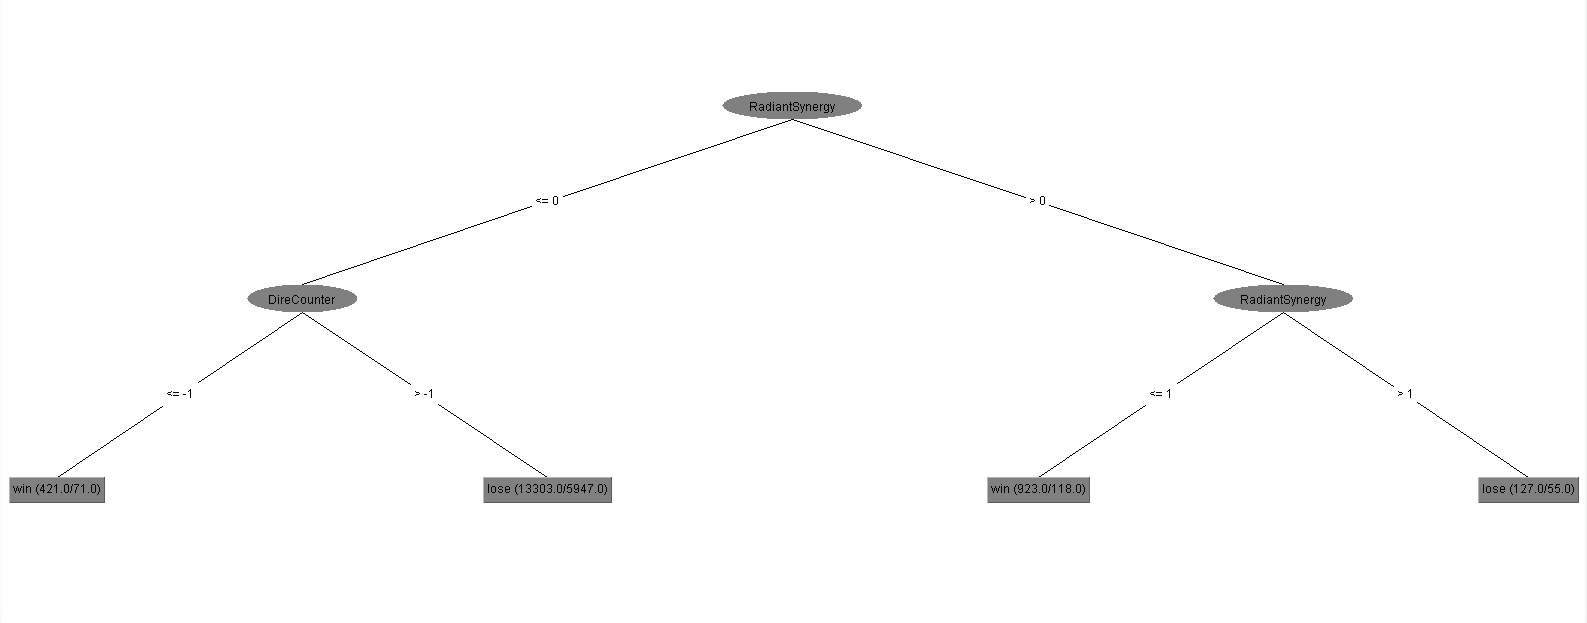
\includegraphics[width=8.0cm]{decisiontree.PNG} 
\newline
\caption{An Example of the Decision Tree}
\label{fig:decisiontree} 
\end{figure}


 The algorithm is proposed by Ross Quinlan~\cite{quinlan}, which is an extension of his earlier ID3 algorithm.

The pseudocode~\cite{Kotsiantis} of the general algorithm for building decision trees by C4.
5 is: 

\begin{enumerate}
\item Check for base cases.

\item For each attribute a, find the normalized information gain ratio from splitting on a.

\item Let a\_best be the attribute with the highest normalized information gain.

\item Create a decision node that splits on a\_best.

\item Recur on the sublists obtained by splitting on a\_best, and add those nodes as the children of the node.

\text{}

\subsubsection{Adaboost}
Adaboost boosting works by combining several relatively
weak and inaccurate classifiers to form a stronger classifier.
In this case, the weak learning algorithm is decision stump,
which consists of a one-level decision tree. Given the decision
stump, train data set and the number of weak classifiers,
k, the adaboost boosting algorithm will produce k weak classifiers
with weights and then combine these weak classifier to
form a stronger classifier based on weights.

\subsubsection{logistic regressing}
Logistic regression is a model that predicts a binary output using a weighted sum of predictor variables. We first trained a simple logistic regression model with an intercept term to
predict the result of a match.

The feature vector we used is described as:
$$ x_i=
\begin{cases}
1& \text{if a radiant player played as the hero with id i}\\
0& \text{otherwise}
\end{cases}$$

Also, the label is defined as:
$$y=
\begin{cases}
1& \text{win the game}\\
0& \text{lose the game}
\end{cases}$$

We divided 90\% of the matches from dataset to form a training set and the remaining 10\% of dataset to form a test set. As the training data becomes larger, the training and test accuracies are coming together closely. We select about 16000 instances as the optimal training set size. 


\begin{figure}[!htbp]
\centering
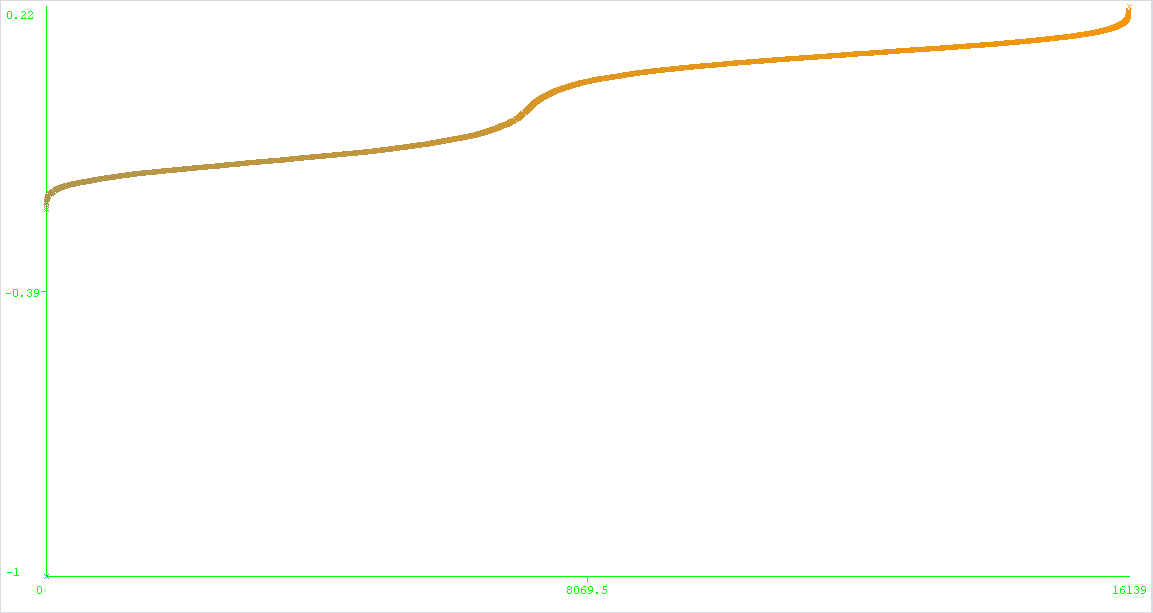
\includegraphics[width=8.0cm]{margincurve.PNG} 
\newline
\caption{Margin Curve of Logistic Regression}
\label{fig:margincurve} 
\end{figure}

This logistic regression model shows that the hero selection is very important to the result of a match. Assuming that all playes have the same game skills, we can predict the result of a set of heroes counter with another set heroes.
However, this only considered the effect of hero set relationships. We also need to analyze the synergy and counter relationship between heroes, which is also a very important factor.

\subsubsection{k-nearest neighbor}
K-nearest neighbors is a non-parametric method for classification and regression that predicts objects’ class memberships based on the k-closest training examples in the feature space. We want to implement K-NN to model the relationship between heros.

To better interpret the relationships between heroes, we run an clustering algorithm to train the synergic and counter relationships. 

\item We randomly select 10 heroes as clustering centers. 

\item Run the K-means clustering algorithm to cluster all 111 heroes into 10 clusters. The distance matric is selected as Euclidean distance.

\item For each clusters, select three nearest neighbors to set up new pairs of relationship.

\item Thus, we get the new 30 pairs of relationships between heroes.

Note that the initial centers are very important to the final clustering results. Also, the synergic relationship is trained by winning games in a same team in a game and the counter relationship is trained by losing games in different teams in a game.


\end{enumerate}


